\chapter{Konzept}

In diesem Kapitel werden das Gesamtkonzept und die Konzepte der einzelnen Tests vorgestellt. Das Gesamtkonzept umfasst die Einzelnen Komponenten von webifier und deren Zusammenspiel. Im Folgenden wird nun das Gesamtkonzept beschrieben.

\section{Gesamtkonzept}

\textit{webifier} ist in viele Unterkomponenten aufgeteilt.
Dies hat den Zweck, bestehende Programme und zukünftige Erweiterungen möglichst getrennt voneinander entwickeln zu können und einzelne Features ab- oder zuzuschalten.
In diesem Abschnitt wird zuerst die Entwurfsarchitektur der Gesamtanwendung erklärt.
Dabei wird hauptsächlich auf den Zweck der Komponenten für die Anwendung und auf deren Zusammenspiel eingegangen.

\begin{figure}[H]
	\centering
	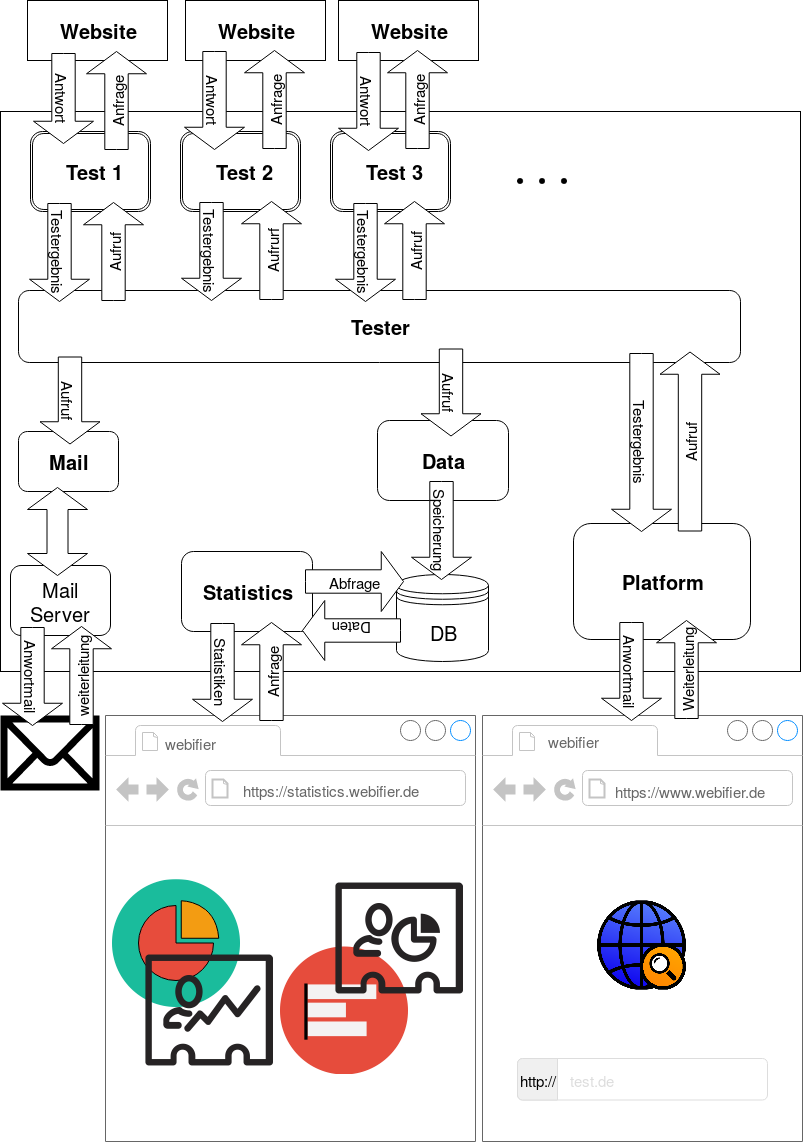
\includegraphics[width=\textwidth]{images/anwendung-konzept}
	\caption{Konzeptarchitektur der Gesamtanwendung}
	\label{fig:anwendung-konzept}
\end{figure}

Grundsätzlich wird webifier benutzt, um Webseiten auf verschiedene Sicherheitsaspekte zu untersuchen.
Abbildung \ref{fig:anwendung-konzept} zeigt den groben Plan der Anwendung.
Es zeigt den konzeptionellen Zusammenhang zwischen den Komponenten, wobei die Datenbank und der Mail Server nicht als eigene Komponenten entwickelt wurden und deshalb keine eigenen Unterabschnitte erhalten.
Die Aufnahme der URLs erfolgt über eine Webseite, die von der Plattform an den Browser des Nutzers ausgeliefert wird.
Die Platform leitet die \ac{URL} aus der Nutzeranfrage an dann an den Tester weiter.
Der Tester ist die Komponente, die die \ac{URL} auf Korrektheit überprüft und ggf. Weiterleitungen auflöst.
Entsteht dabei ein Fehler, so wird dieser an die Platform porpagiert und schließlich im Browser angezeigt.
Wurde die Auflösung der \ac{URL} erfolgreich ausgeführt, werden die Sicherheitstests gestartet.

Eine weitere Möglichkeit, webifier zu verwenden, ist über Mailverkehr.
Hat der Nutzer eine Spam-verdächtige E-Mail in seinem Postfach, so kann er diese an ein bestimmtes Postfach von webifier weiterleiten.
Dort werden Links  aus der Mail zusammengetragen und an den Tester weitergeleitet.

Im Tester wird die Ausführung der einzelnen Tests gestartet, überwacht und koordiniert.
Wichtig dabei ist, dass alle Tests abgeschottet vom Rest des Systems laufen, da auf ihnen schadhafte Webseiten aufgerufen werden.
Es können beliebig viele Tests im Tester hinzugefügt werden, indem sie in der Konfiguration angegeben werden.
Jeder dieser Tests gibt ein eigenes Ergebnis, sowie weitere Informationen zurück.
Diese Ergebnisse werden dann miteinander verrechnet und es wird eine Gesamteinschätzung zusammen mit allen relevanten Informationen der einzelnen Tests ausgegebe.

Alle Ergebnisse der Tests werden anhand von Schwellwerten und Gewichtungen ausgerechnet, wobei die Anwendung zwischen vier Ergebnistypen unterscheidet: \textit{CLEAN}, \textit{SUSPICIOUS}, \textit{MALICIOUS} und \textit{UNDEFINED}.

\begin{description}
    \item[unbedenklich] \hfill \texttt{CLEAN} \\
    Die Webseite verhält sich harmlos und ist ungefährlich.
	\begin{figure}[H]
		\centering
		
\includegraphics[scale=0.2]{images/webifier-clean}
		\caption{Icon für den Testergebnistyp \textit{CLEAN}}
	\end{figure}

	\item[verdächtig] \hfill \texttt{SUSPICIOUS} \\
	Die Webseite verhält sich bedenklich und ist suspekt.
	Diese Seite sollte gemieden werden.
    \begin{figure}[H]
    	\centering
    	
\includegraphics[scale=0.2]{images/webifier-suspicious}
    	\caption{Icon für den Testergebnistyp \textit{SUSICIOUS}}
    \end{figure}

    \item[bedrohlich] \hfill \texttt{MALICIOUS} \\
    Die Webseite verhält sich kritisch und ist gefährlich.
    Sie sollte unter keinen Umständen aufgerufen werden.
    \begin{figure}[H]
    	\centering
    	
\includegraphics[scale=0.2]{images/webifier-malicious}
    	\caption{Icon für den Testergebnistyp \textit{MALICIOUS}}
    \end{figure}

	\item[unbekannt] \hfill \texttt{UNDEFINED} \\
	Der Test konnte aus technischen oder zeitlichen Gründen nicht vollendet werden.
	Es kann keine Aussage über die Bös- oder Gutartigkeit der Seite gemacht werden.
	\begin{figure}[H]
		\centering
		
\includegraphics[scale=0.2]{images/webifier-undefined}
		\caption{Icon für den Testergebnistyp \textit{UNDEFINED}}
	\end{figure}
\end{description}

Das berechnete Gesamtergebnis des Testers wird an die webifier Platform bzw. an webifier
Mail weitergeleitet. Schließlich wird das Ergebnis dem Nutzer über den Browser bzw. über eine
Antwortmail präsentiert. Zusätzlich werden alle Ergebnisse des Testers an webifier Data geschickt
und dort in einer Datenbank persistiert. Diese Daten werden von webifier Statistics für Analysen und
Auswertungen genutzt

\subsection{webifier Tests}
Webifier Tests ist der Oberbegriff für sämtliche von webifier durchgeführten Tests bei der Analyse einer Webseite. Wie bei der gesamten Anwendung wird auch bei den Tests viel Wert auf Modularität gelegt. Jeder Test bildet ein eigenständiges Bauteil, welches nach belieben integriert oder entfernt werden kann ohne Effekte auf die Lauffähigkeit der Gesamtanwendung.

Da webifier auf die Analyse von maliziösen Seiten ausgelegt ist gibt es bei den Tests einige Punkte zu beachten um das System vor Viren und Schadcode zu schützen.
Jeder Test wird in einer vom Gesamtsystem abgekapselten Laufzeitumgebung ausgeführt. Aus einem Test heraus darf nicht auf das System zugegriffen werden, da die Tests gegebenenfalls mit Schadcode befallen werden können durch das Erforschen von maliziösen Seiten. Es soll vermieden werden, dass sich Schadcode oder Viren von den Tests auf den Server verbreiten. Nach Durchlauf und Übermittelung des Ergebnisses löscht der Test sich selbst und alle Laufzeitdaten. Als Ergebnis werden keinerlei Dateien versendet, es beschränkt sich auf eine Weitergabe des Ergebnisses in Form einer Zeichenkette. Damit soll vermieden werden, dass sich eventuell mit Viren befallene Dateien weiter auf dem System ausbreiten können.

Ein Test liefert sein Ergebnis an den Tester, welcher dies dann im folgenden weiterverarbeitet.
Das Starten und Organisisieren der Tests wird von webifier Tester durchgeführt. Den Aufbau und die Funktionsweise des Testers wird im nächsten Abschnitt beschrieben. Zum Starten eines Tests werden zwei Startparameter mitgegeben. Zum Einen wird die ID zur Identifikation mitgegeben und zum anderen die vollständig aufgelöste URL der zu testenden Seite.
 
Webifier stellt 9 verschiedene Tests um eine Webseite zu überprüfen. Das Konzept der einzelnen Test wird in jeweils eigenständigen Kapiteln erläutert. Hier folgt noch ein Überblick über die einzelnen Tests.

\begin{table}[H]
\centering
\begin{tabular}{|l|l|l|l|}
\hline
\textbf{Test} & \textbf{Beschreibung} \\\hline
Virenscan der Webseite & Testet die Dateien einer Seite auf Viren \\\hline
Vergleich in verschiedenen Browsern & Test ob sich die Seite bei verschiedenen \\ & Browsern anders verhält \\\hline
Überprüfung der Port-Nutzung & Überprüft ob die Seite Portscanning betreibt \\\hline
Überprüfung der IP-Nutzung & Überprüft ob die Seite IPScanning betreibt \\\hline
Prüfung aller verlinkten Seiten & Testet die Links auf der Webseite gegen die \\ & Datenbank von webifier \\\hline
Google Safe Browsing & Nutzt die Google-API um die Webseite von \\ & Google testen zu lassen \\\hline
Überprüfung des SSL-Zertifikats & Überprüft das SSL-Zertifikat der Webseite \\\hline
Erkennung von Phishing & Testet ob es sich um eine Phishingseite handelt \\\hline
Screenshot der Seite & Gibt dem Nutzer einen Screenshot der Webseite \\\hline
\end{tabular}
\caption{Beschreibung der einzelnen Tests}
\label{tbl:tests}
\end{table}

\subsection{webifier Tester}
\label{sec:konzept-tester}

Der webifier Tester verwaltet alle Tests, führt diese aus und berechnet aus den einzelnen Ergebnissen der Tests ein Gesamtergebnis. Alle auszuführenden Tests werden in einer Konfigurationsdatei angegeben und können deshalb dynamisch angepasst werden. Da jeder Test in einem eigenen Prozess läuft wird beim Starten des Testers die Konfigurationsdatei geladen. Anschließend werden die einzelnen Tests ausgeführt und auf ein Ergebnis gewartet. Liegt von allen Tests das Ergebnis vor wird ein Gesamtergebis berechnet. Die Berechnung dieses Ergebnisses wird im Folgenden genauer erklärt.

Das Ergebnis kann entweder unbedenklich (\textit{CLEAN}), verdächtig (\textit{SUSPICIOUS}), bedrohlich (\textit{MALICIOUS}) oder unbekannt (\textit{UNDEFINED}) sein. Für die Berechnung des Endergebnisses erhält jeder Test wie in Tabelle \ref{tbl:test-weights} dargestellt eine Gewichtung, da einige Tests mehr über die Vertrauenswürdigkeit oder Gefahr einer Webseite aussagen als andere. Am meisten fallen der \textit{Virenscan der Webseite} und die \textit{Erkennung von Phishing} ins Gewicht, da dieses die ausschlaggebendsten Tests sind. Am wenigsten gewichtet sind der \textit{Vergleich in verschiedenen Browsern}, weil dies nur ein Indiz ist, da es auch viele Webseiten, wie die von YouTube, Nachrichtensendern, Blogs oder Ähnlichem gibt, welche immer dynamischen Inhalt bereitstellen und die \textit{Prüfung der verlinkten Seiten}, da dies immer vom Datenbestand abhängt. Der \textit{Screenshot der Seite} fällt nicht ins Gewicht, da dies kein Test im eigentlichen Sinne ist, sondern nur eine zusätzliche Information für den Nutzer darstellt. In Abschnitt \ref{sec:konzept-testarten} wird die Wahl der Gewichtungen für die einzelnen Tests noch ausführlicher erläutert.

\begin{table}[H]
\centering
\begin{tabular}{|l|l|l|l|}
\hline
\textbf{Test} & \textbf{Gewichtung} & \textbf{Prozentuale Gewichtung} \\\hline
Virenscan der Webseite & 5 & \textasciitilde0,208\\\hline
Vergleich in verschiedenen Browsern & 1 & \textasciitilde0,042\\\hline
Überprüfung der Port-Nutzung & 3 & 0,125\\\hline
Überprüfung der IP-Nutzung & 3 & 0,125\\\hline
Prüfung aller verlinkten Seiten & 1 & \textasciitilde0,042\\\hline
Google Safe Browsing & 3 & 0,125\\\hline
Überprüfung des SSL-Zertifikats & 3 & 0,125\\\hline
Erkennung von Phishing & 5 & \textasciitilde0,208\\\hline
Screenshot der Seite & 0 & 0\\\hline
\end{tabular}
\caption{Gewichtungen der einzelnen Tests}
\label{tbl:test-weights}
\end{table}

Die prozentuale Gewichtung ergibt sich aus $\frac{Testgewichtung}{Summe~der~Gewichungen~aller~Tests}$.

Ein weiterer wichtiger Punkt, der für die Berechung ges Gesamtergebnisses festgelegt wurde ist, dass mindestens 50\% aller Tests (berechnet anhand der prozentualen Gewichtung) ein bekanntes Ergebnis, also \textit{CLEAN}, \textit{SUSPICIOUS} oder \textit{MALICIOUS} haben müssen. Ist der Anteil bekannter Ergebnisse kleiner lässt sich kein zuverlässiges Ergebnis berechnen, da dieses sonst von zu wenigen ausschlaggebenden Faktoren abhängen würde.

Liefern also mehr als die Hälfte der Tests ein bekanntes Ergebnis, so kann daraus nun das Gesamtergebnis berechnet werden. Hierfür wird für jedes Testergebnis ein Wert zwischen 0 und 1 berechnet, welcher anschließend mit der prozentualen Gewichtung des Tests multipliziert wird. Die Werte der einzelnen Testergebnisse ergeben sich wie in Tabelle \ref{tbl:test-values} dargestellt. Ist das Testergebnis \textit{CLEAN} oder \textit{UNDEFINED} ist der Ergebniswert 0 und geht so nicht weiter in die Wertung ein. Ist das Ergebnis \textit{MALICIOUS} wird der Wergebniswert 1. Dadurch Fällt das Gewicht dieses Tests voll in die Wertung. Ist das Ergebnis \textit{SUSPICIOUS} so wird die prozentuale Gewichtung des Tests als Ergebniswert gewählt. So fließt dieser Test mit dem Quadrat der Gewichtung in das Gesamtergebnis ein.

\begin{table}[H]
\centering
\begin{tabular}{|l|l|l|l|}
\hline
\textbf{Testergebnis} & \textbf{Ergebniswert}\\\hline
\textit{CLEAN} & 0\\\hline
\textit{SUSPICIOUS} & Prozentuale Gewichtung des Tests\\\hline
\textit{MALICIOUS} & 1\\\hline
\textit{UNDEFINED} & 0\\\hline
\end{tabular}
\caption{Zuordnung Testergebnis zu Ergebniswert}
\label{tbl:test-values}
\end{table}

Anschließend werden die Werte aller Tests zu einem Endergebnis aufsummiert. Daraus ergibt sich im Gesamtergebnis ein Minimalwert von 0 und ein Maximalwert von 1. Dieser Wertebereich wird nun wie folgt auf die drei Ergebnisse \textit{CLEAN}, \textit{SUSPICIOUS} und \textit{MALICIOUS} verteilt. Die Tests mit der größten Gewichtung sollen hierbei ausschlaggebend sein. Daraus ergibt sich die prozentuale Gewichtung des Tests mit der größten Gewichtung als Minimalwert für \textit{MALICIOUS} und das Quadrat der prozentualen Gewichtung des Tests mit der größten Gewichtung als Minimalwert für \textit{SUSPICIOUS}.

Daraus lässt sich für die Werte der Tests aus Tabelle \ref{tbl:test-weights} die folgende Werteverteilung der Gesamtergebniswerte ableiten:

\begin{center}
$0 \leq CLEAN < 0,043402\overline{7} \leq SUSPICIOUS < 0,208\overline{3} \leq MALICIOUS \leq 1$
\end{center}

Zusätzlich zu dem berechneten Gesamtergebnis stellt der Tester auch alle Ergebnisse der Einzeltests und deren spezifischen Testinformationen bereit. Außerdem werden alle Ergebnisse zu Persistierung an das Modul webifier Data gesendet, welches in Abschnitt \ref{sec:konzept-data} genauer erläutert wird.

\subsection{webifier Plattform}

webifier Plattform ist eine Webanwendung, die auf den Tester aufsetzt und eine \ac{UI} für diesen zu Verfügung stellt. Außerdem bereitet sie die Ergebnisse des Testers grafisch für den Benutzer auf.

Der Nutzer hat die Möglichkeit auf der ersten Seite von webifier Plattform eine Url einzugeben, welche getestet werden soll. Da die Kapazität jedes Systems beschränkt ist verwaltet die Plattform alle Anfragen zur Webseitenüberprüfung in einer Warteschlange. In einer Konfigurationsdatei kan angegeben werden, wie viele Tests parallel ausgeführt werden sollen. So wird die Warteschlange nach und nach abgearbeit und anschließend werden die Ergebnisse des Testers für den Benutzer visuell aufbereitet. Das bereitgestellte Ergebnis umfasst zum Einen das Gesamtresultat, welches vom Tester berechnet wurde und zu Anderen sowohl die Ergebnisse der einzelen Tests, als auch die Zusätzlichen Informationen, welche von diesen bereitgestellt wurden.

So erhält der Nutzer einen umfassenden Bericht über die Vertrauenswürdigkeit oder die ausgehende Gefahr der überprüften Webseite.

\subsection{webifier Mail}
Diese Komponente ist ein Zusatzfeature, mit dem verdächtige Mails über den webifier Tester überprüft werden können. Nutzer müssen dazu lediglich ihre empfangene Mail an für \textit{webifier Mail} bereitgestelltes Postfach weiterleiten. In \textit{webifier Mail} werden dann bis zu fünf in der Mail enthaltene Links an den Tester weitergeleitet. Ist die Prüfung vollendet wird eine Antwortmail mit den Ergebnissen an den Nutzer zurückgeschickt.

\subsection{webifier Data}
\label{sec:konzept-data}

webifier Data ist die Persistenzkomponente von webifier. webifier Tester nutzt webifier Data um alle Testergebnisse an einem zentralen Ort abzulegen, egal wo dieser ausgeführt wird.

Ein Testergebnis, welches in dem Datamodul gespeichert wird enthält einmal die eingegebene Url und die getestete Url, das Gesamtergebnis, sowohl den Typ (\textit{CLEAN}, \textit{SUSPICIOUS}, \textit{MALICIOUS} oder \textit{UNDEFINED}), als auch den Ergebniswert. Außerdem wird die Testlaufzeit gespeichert. Zusätzlich werden noch weitere Informationen zu den einzelnen Tests gespeichert. Dazu zählen der Name, die Konfigurationsparameter, wie beispielsweise die Gewichtung, das Resultat und die Detailinformationen zu diesem.

Die Komponente stellt auch eine Schnittstelle zum Abfragen der bereits gespeicherten Ergebnisse bereit. Diese wird beispielsweise vom Test \textit{Prüfung aller verlinkten Seiten} verwendet. Die Funktionsweise dieses Tests wird in Abschnitt \ref{sec:konzept-linkchecker} erklärt.

Alle Ergebnisse werden in einer Datenbank abgelegt. Da die zusätzlichen Informationen der einzelnen Tests teilweise sehr unterschiedlich sind, kommt hierfür keine relationale Datenbank in Frage. webifier Data nutzt deshalb zur Speicherung aller Daten die Dokument basierte Datenbank MongoDB. Alle weiteren Informationen hierzu folgen im Umsetzungsteil dieser Arbeit.

\subsection{webifier Statistics}
Webifier Statistics ist die Statistikoberfläche von webifier. Hier werden alle Daten der analysierten Webseiten aufbereitet und in visueller Form dargestellt. Die Daten stammen aus den Ergebnissen aller Tests, welche von webifier Data abgespeichert wurden.

Webifier Statistics liefert dem Nutzer eine Vielzahl an verschiedenen Graphen, welche bestimmte Teilaspekte beleuchten. Diese enthalten zum Einen die Gesamtauswertungen, welche sich mit der allgemeinen Datenauswertung jedes Gesamttests beschäftigen. Zum Anderen gibt es noch die Einzelauswertungen der Tests, die testspezifische Ergebnisse auswerten.

Alle Auswertungen werden dem Nutzer über eine Weboberfläche zugänglich gemacht. Als Einstieg gibt es ein \textit{Dashboard} mit einigen Zahlen und Fakten zu den Aktivitäten auf webifier. Auf die einzelnen Auswertungen wird in der Auswertung genauer eingegangen.

\section{Testarten}
\label{sec:konzept-testarten}

In diesem Abschnitt werden nun die einzelnen Tests vorgestellt, mit welchen die zu überprüfende Webseite analysiert wird. Wie bereits erwähnt werden alle dieser Tests vom Tester verwaltet und ausgeführt.

\subsection{Virenscan der Webseite}

Der Virenscan der Webseite führt nutzt verschiedene Virenscanner um die Webseite auf Malware zu überprüfen. Um dies zu realisieren wird zunächst die Webseite inklusive aller enthaltenen Dateien und Links heruntergeladen und gespeichert. Anschließend werden die Virenscanner gestartet, welche die heruntergeladenen Dateien überprüfen. Abschließend werden alle Ergebnisse der einzelnen Scans zusammengeführt und daraus ein Endergebnis berechnet.

Für das Endergebnis werden zunächst alle gescannten Dateien klassifiziert. Wird eine Datei von keinem der Virenscanner als Malware eingestuft wird diese als \textit{CLEAN} gekennzeichnet. Klassifiziert nur ein Virenscanner die Datei als Malware, wird diese also \textit{SUSPICIOUS} eingestuft. Halten mehr als ein Virenscanner eine Datei für Malware ist diese \textit{MALICIOUS}. Sind alle Dateien als \textit{CLEAN} eingestuft, so ist auch das Endergeblis dieses Tests \textit{CLEAN}. Sollten ein oder mehrer Dateien \textit{SUSPICIOUS} sein wird auch das Endergebnis \textit{SUSPICIOUS}. Das selbe gilt danach für \textit{MALICIOUS}. Sobald eine Datei \textit{MALICIOUS} ist, ist das Endergbnis ebenfalls \textit{MALICIOUS}.

Zusätzlich zum Endergebnis wird noch die gesamte Liste der gescannten Dateien inklusive der jeweiligen Klassifizierung bereitgestellt und vom Tester weitergegeben.

\subsection{Vergleich in verschiedenen Browsern}

In \autoref{sec:user-agent-sniffing} wurde bereits das Thema \textit{User Agent Sniffing} behandelt.
Dieser Test soll genau dieses Problem aufgreifen.
Es sollen \ac{HTTP}-Anfragen von verschiedene Browsertypen mit entsprechenden User Agents an den Webserver der Zielseite geschickt werden.
Danach werden die Antworten untereinander auf Unterschiede untersucht. Dabei entstehen Kennwerte für die Übereinstimmung der Antworten, die miteinander verrechnet werden müssen.
Dieser berechnete Wert für die Durchschnittsübereinstimmung muss schließlich anhand von passenden Schwellwerten die richtige Ergebnisklasse eingeteilt werden.

\subsection{Überprüfung der Port-Nutzung}
Der Test auf Port Scanning analysiert die Nutzung der Ports einer Webseite. Hierfür wird die Webseite automatisch vom Test geöffnet und dessen JavaScript ausgeführt. Parallel dazu muss die Netzwerkaktivität überwacht werden. Es werden alle eingehenden Anfragen auf das Testsystem zunächst geloggt. Da das Testsystem abgekapselt vom restlichen System ist, ist es irrelevant von welcher IP-Adresse die Anfragen kommen. Alle Anfragen lassen sich auf die aufgerufene Seite zurückführen, da restliche Netzwerkaktivität abgeschaltet ist. Dies ist wichtig, da es durchaus möglich ist das die Webseite nicht selbst einen Portscan-Angriff startet sondern beispielsweise über einen Drittrechner oder ein Botnetz gescannt wird. Zudem könnten die Ports auch lokal auf dem Client über JavaScript gescannt werden. Deshalb werden lediglich die angefragten Ports im Log gespeichert.

Nach erfolgreichem Durchschauen der Webseite beginnt die Analyse. Hier müssen alle Portanfragen klassifiziert werden. Es gibt eine Reihe von legitimen Portanfragen welche beispielsweise Port 80 für HTTP oder Port 443 für SSL sind. Diese Anfragen werden dann als harmlos markiert und somit ignoriert. Alle Anfragen, welche sich auf unspezifizierte Ports beziehen, werden als verdächtig markiert. Je nach Anzahl der verdächtigen Anfragen wird dann entschieden ob die Seite als bedrohlich, verdächtig oder sauber klassifiziert wird. Dieses Ergebnis wird dann mitsamt der gefundenen verdächtigen Portanfragen zurückgegeben.

\subsection{Überprüfung der IP-Nutzung}
Der Test auf IP Scanning beschäftigt sich mit der Analyse der IP-Anfragen, welche durch eine Webseite ausgelöst werden. Wie auch bereits bei Portscanning beschrieben wird die Webseite automatisch geöffnet und dessen JavaScript ausgeführt. Die Netzwerküberwachung hat hier jedoch einen anderen Fokus. Es werden die IPs der gesendeten Anfragen geloggt. Beim IP Scanning wird grundsätzlich versucht über die bekannten Heimnetz-IP-Netze weitere im Netzwerk angeschlossene Geräte zu erkennen um beispielsweise Viren auf dem gesamten Netzwerk zu verbreiten. Diese Angriffe werden über JavaScript auf dem Clienten gestartet. Deshalb werden die vom Clienten gesendeten Anfragen protokolliert. Hiervon werden lediglich die IPs gespeichert.

Nach dem Speichern aller IPs werden diese klassifiziert. Der Test vergleicht alle Anfragen mit den bekannten Heimnetz-IPs (beispielsweise 192.168.178.*). Anfragen, welche sich nicht auf diese Adressen zurückführen lassen werden herausgefiltert, da diese irrelevant für den Test sind. Anhand der Anzahl der verdächtigen Adressen wird im Abschluss wieder die Seite klassifiziert und das Ergebnis mitsamt den Adressen zurückgeliefert an den Tester.

\subsection{Prüfung aller verlinkten Seiten}
\label{sec:konzept-linkchecker}

Dieser Test sucht innerhalb des Quellcodes der Anwendung nach Hyperlinks und referenzierten Ressourcen.
Für alle gefundenen Hosts wird dann prüft, ob bereits Einträge dazu in der Datenbank unter webifier Data vorhanden sind.
Gibt es einen Eintrag, der \textit{SUSPICIOUS} ist, dann ist das ganze Endergebnis \textit{SUSPICIOUS}.
Falls jedoch mehr als 34\% der Hosts \textit{UNDEFINED} sind, dann ist auch das Gesamtergebnis \textit{UNDEFINED}.
Sobald ein Eintrag \textit{MALICIOUS} ist, so ist auch das Gesamtergebnis \textit{MALICIOUS}.
Ansonsten liefert der Test \textit{CLEAN} zurück.

\subsection{Google Safe Browsing}

\begin{quote}
	Safe Browsing is a Google service that lets client applications check URLs against Google's constantly updated lists of unsafe web resources.\footcite[Vgl.][]{googleSafeBrowsing}
\end{quote}

Dieser Cloud-Service erlaubt es der Anwendung also eine weitaus größere Datenbank als ihre eigene anzuzapfen.

Der Service unterscheidet zwischen vier Bededrohungstypen\label{par:konzep-gsb-types}: Malwareseiten, Sozialmanipulationsseiten, ungewollte Software und potenziell schadhafte Webanwendungen.
Weitere Vorteile sind die Autorität des Unternehmens und die einfach zu bewerkstelligende Integration des Services.
Leider können die Einträge aus der Datenbank des Services nicht exportiert werden, sondern können nur gegen Listen von Links gecheckt werden.
In diesem Test werden wie bei der Prüfung der verlinkten Seiten alle Links zu Webseiten und Resourcen zusammengetragen.
Diese werden dann aber nicht an webifier Data, sondern an den Google Safe Browsing Dienst weitergeleitet.
Sobald ein Treffer aus dem Service zurückgemeldet wird, ist das Ergebnis \textit{SUSPICIOUS}.
Falls sich mehr als 40\% der Links in der Datenbank befinden, so wird die Webseite als \textit{MALICIOUS} eingestuft.
Ist die zu testende Webseite selbst ein Match, so ist das Ergebnis ebenfalls \textit{MALICIOUS}.
Wird kein Eintrag gefunden, dann zählt die Seite als \textit{CLEAN}.

\subsection{Überprüfung des SSL-Zertifikats}

Die Überprüfung des SSL-Zertifikats der Weibseite sucht nach einem vorhandenen Zertifikat und validiert dieses, sofern die Webseite eines nutzt. Hierfür liest es die dafür notwendigen Informationen des  Zertifikats aus und berechnet anschließend ein Testergebnis.

Stellt die Webseite kein Zertifikat zur Verfügung so ist das Testergebnis \textit{SUSPICIOUS}, da es in Zeiten von Let's Encrypt\footnote{\url{https://letsencrypt.org/}} jedem möglich ist ein SSL-Zertifikat kostenlos zu erwerben und so die Sicherheit der eigenen Webseite zu erhöhen. Nutzt die Webseite ein valides Zertifikat ist das Ergebnis \textit{CLEAN}. Weist das Tertifikat Fehler auf ist das Ergebnis \textit{MALICIOUS}. Solche Fehler können beispielsweise sein, dass das Zertifikat abgelaufen ist, dass es selbst signiert wurde oder das es für den falschen Host genutzt wird.

\subsection{Erkennung von Phishing}

webifier enthält auch einen sehr einfachen Test zur Erkennung von Phishing. Dieser sucht zuerst nach den Schlagwörtern der gegebenen Webseite. Hierfür zählt er die Häufigkeit aller vorkommenden Wörter die mehr als drei Buchstaben haben. Wörter in Bildbeschreibungen und Überschriften werden doppelt gewichtet, Wörter im Titel der Webseite werden fünffach gewichtet. Haben mehere Wörter die gleiche Gewichtung, so fällt die Länge der Wörter auch noch ins Gewicht und längere Wörter werden bevorzugt. Die vier Wörter, die im Ranking am höchsten stehen werden anschließend als Schüsselwörter gewählt.

Anschließend werden mit Hilfe öffentlicher Suchmaschinen mögliche Duplikate der Webseite gesucht. Für diese Suche werden die ausgewählten Schlagwörter verwendet. Nun werden die Ergebnisse aller Suchmaschinen zusammengeführt und ebenfalls gewichtet. Je mehr Suchmaschinen einen Link gefunden haben, desto höher steigt dieser Link im Ranking. Als nächstes muss diese Liste der möglichen Duplikate nach Orginalen, welcher der gegebenen Webseite entsprechen gefilterert werden, da es sehr wahrscheinlich ist, dass diese ebenfalls in der Liste der Links enthalten ist. Als letztes wird die Liste noch auf maximal zehn Eintrage gekürtzt.

Nun werden alle gefundenen Links mit der gegebenen Webseite verglichen und für jeden gefundenen Link ein Ergebnis berechnet. Der Vergleich erfolgt auf drei Ebenen: es werden der Inhalt und er der Quelltext der beiden Webseiten, aber auch das Aussehen verglichen. Jeder dieser Vergleiche gibt die prozentuale Übereinstimmung der zu vergleichenden Webseiten zurück. Anschließend werden diese drei Ergebnisse zu einem Gesamtergebnis verrechnet. In diese Rechnung fließt das Ergebnis des Screenshotsvergleichs mitt doppeltem Gewicht ein, da dieser Vergleich am aussagekräftigsten ist.

Aufgrund der Komplexität wird die genaue Berechnung des Ergebnisses wird in Abschnitt \ref{sec:umsetzung-phishungdetector} erklärt und hier nun vereinfacht dargestellt. Stimmen die beiden Webseiten zu 80\% überein, so ist das Ergebnis des Links \textit{SUSPICIOUS}, stimmen die beiden Webseiten zu 90\% überein, so ist das Ergebnis \textit{MALICIOUS}. Das Endergebnis des Tests wird abschließend wie folgt berechnet: wurde mindestens ein verdächtiger Link gefunden, so ist das Gesamtergebnis \textit{SUSPICIOUS}, wurde mindestens ein bedrohlicher Link gefunden, so ist das Ergebnis \textit{MALICIOUS}, andernfalls \textit{CLEAN}. Zusätzlich werden noch die gefundenen Schlagwörter, die gefundenen Phishingseiten, derern Vergleichswerte und ein Überlagerungsscreenshot mit der Originalseite für den Tester bereitgestellt.

\subsection{Screenshot der Seite}
Der Screenshot-Test ist kein Test im eigentlichen Sinne. Er liefert keine Aussage über die Bedrohlichkeit einer Webseite. Deshalb liefert er immer als Ergebnis sauber und bleibt ungewichtet in der Gewichtung im Tester. Trotzdem wurde er mit implementiert um den Nutzern einen Blick auf die Seite zu geben, welche sie von webifier haben scannen lassen. Dies kann besonders interessant sein, da viele Nutzer auch daran interessiert sind wie die Seiten denn aussehen und was dort an Text oder Bilder zu sehen ist. Jedoch sollte keiner der Nutzer, auf eine als bedrohlich markierte Webseite, mit seinem Webbrowser zugreifen. Deshalb wird hier die Möglichkeit gegeben sich gefahrlos einmal die Webseite anzuschauen.
